\section{Experiments And Results}
\label{sec:evaluation}
As described in section \ref{sec:visual-aspects} \emph{deep dreaming} works by selecting layers and neurons that should be activated more.
In order to select good layers for the dreaming, we let each layer be dreamt onto an image to handpick the layers that offer interesting features.
Impressive results of that can be seen in section \ref{sec:withoutguide}.

To get a more granular control of the intensified features, one can use a guide image.
A guided dream, described in section \ref{guided-dreaming}, will select neurons based on the guide image in that layer.
The results are presented in section \ref{sec:withguide}.


\subsection{Performance Considerations}
\label{sec:performance}
The runtime of the deep dream depends mostly on the size of the input image and the layer amount.
Using an image of $\approx$600x430 pixels, 30 layers, 10 iterations and 4 octaves can already take around 45 minutes to apply and uses up to 14GB of RAM\footnote{single threaded i7-5930k@3,5GHz, 32GB RAM}.
We also implemented the bilateral filter which will be applied after every step.\cite{bilateral}
This will also heavily slow down the runtime because the application of the filter takes a few seconds and is applied at every step of modification.


\subsection{Without Guide Image}
\label{sec:withoutguide}

As mentioned in section \ref{sec:data}, the analyzed model contains 50 layers, so we will not be showing the results for each one, but rather a selection that we deemed satisfactory.
Throughout these layers one can find all kinds of features varying from different colors, textures to small parts of objects.
Looking at (TODO: layer 15/18 + 13/14) one can see that the recognizable features within a layer are definitely not limited to a particular one and also includes transitions(layer 13/14).
These transitions can either distinguish pixelated regions to very sharp ones.
But it can also result in a transition from smooth curves to very straight lines (layer16/18).
Going further up in the layers we found one layer of particular interest, depicted in figure \ref{fig:layer-snake}.
It visualizes four distinct things at once which makes it unique.
There is a snake's head in the lower left part of the image as well as to the right of the very left house.
The field and large parts of the sky were transformed to look like snake scales.
Apart from these two already distinctive objects the center seems to contain the right part of a dog's face and above the sky looks more like dog fur than snake scales.  
If one looks for definite objects one can find eyes TODO: (layer 43), dogs(layer), 

Another interesting find is layer 12 depicted in figure \ref{fig:layer-artistic}.
If one ignores the lines and purple tint it looks like an artistic style filter was applied.
This supports DiPaolo's findings, mentioned in section \ref{sec:previous-work}, that by using the right combination \textit{deep dream} can be used to modify pictures such that they look like paintings.

Another applied change that can be observed in almost all layers is a slight purple to rainbowish tint that gets applied to the image, especially around the newly added features, as visible within the lines in figure \ref{fig:layer-artistic} and in the sky of figure \ref{fig:layer-snake}.

\begin{figure}[H]
	\centering
	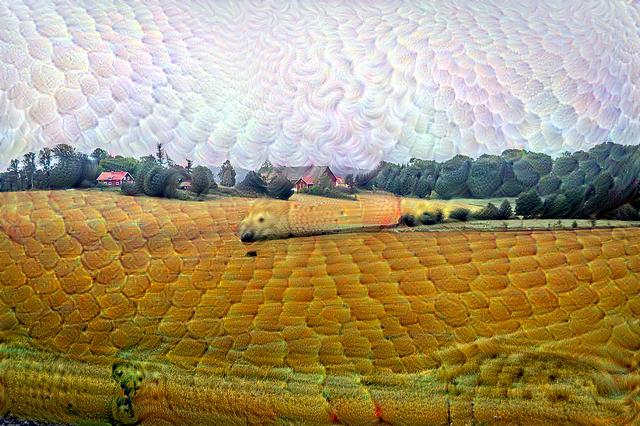
\includegraphics[width=0.7\linewidth]{img/alpsted-landscape_res4f_branch2a.jpg}
	\caption{Layer 41 \emph{res4f\_branch2a}. Seems like snake scales with a snake head in the lower left.}
	\label{fig:layer-snake}
\end{figure}
\begin{figure}[H]
\centering
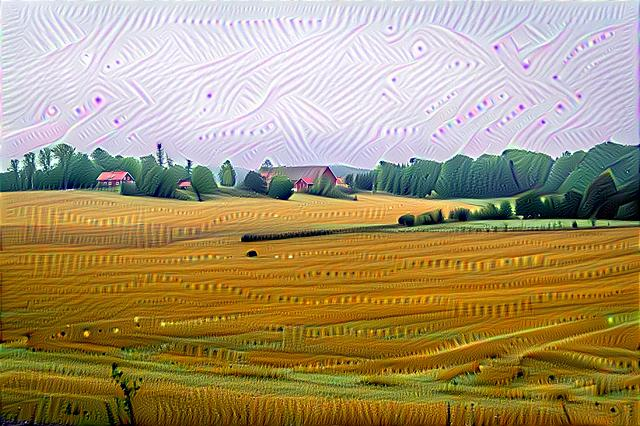
\includegraphics[width=0.7\linewidth]{img/alpsted-landscape_res3a_branch1.jpg}
\caption{Layer 12 \emph{res3a\_branch1}. Apart from the distinct lines it seems to apply an artistic filter.}
\label{fig:layer-artistic}
\end{figure}


%TODO: beispiel hohe stepsize => visualisierung von haus o.a.
\subsection{With Guide Image}
\label{sec:withguide}

\subsection{Repeating Features}
\label{sec:repeating-features}

Within the different layers we found some to behave quite similar.
Previously we presented layers that differ from each other in form, size and shape.
Here we present layers that seem to have learned almost the same features.
To show the behavior in the clearest way possible we applied dreaming onto the same random generated noise.
As one can see in the figures \ref{fig:rotated_feature_1} \ref{fig:rotated_feature_2}, the created images look almost the same, the only real difference is the orientation.
It looks the enhanced features were simply rotated.

\begin{figure}[H]
	\minipage{0.49\textwidth}
	\centering
	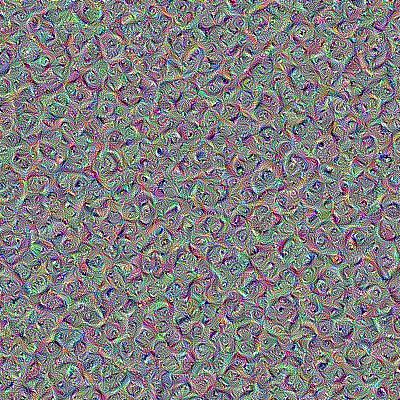
\includegraphics[width=1\linewidth]{img/rotated_feature_1.jpg}
	\caption{Dreamed onto random now with the \enquote{res2c\_branch2b} layer}
	\label{fig:rotated_feature_1}
	\endminipage\hfill
	\minipage{0.49\textwidth}
	\centering
	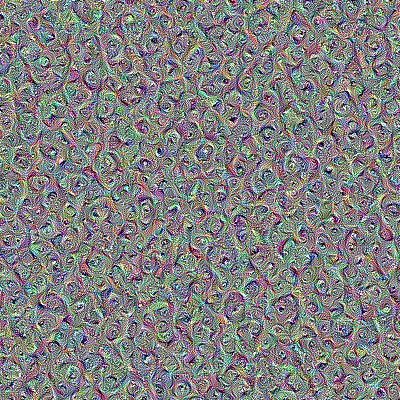
\includegraphics[width=1\linewidth]{img/rotated_feature_2.jpg}
	\caption{Dreamed onto random now with the \enquote{res2c\_branch2c} layer}
	\label{fig:rotated_feature_2}
	\endminipage\hfill
\end{figure}

